\section{Experiments}
\label{sec:exp}

In the following experiments, we train all scenes using the original Gaussian Splatting implementation~\citep{kerbl2023gaussiansplatting} with default hyperparameters. To reduce memory usage, half of the Gaussians are filtered out based on their importance, as described in Sec.~\ref{sec:uplifting}.

We uplift features from DINOv2 ViT-g with registers~\citep{darcet2024registers}, SAM~\citep{kirillov2023sam}, SAM 2~\citep{ravi2024sam2}, and OpenCLIP ViT-B/16~\citep{ilharco2021openclip}.
%
Key parameters (\eg the segmentation threshold and the definitions of $S_f$ and $P$ in graph diffusion) are either fixed across all scenes of a task or automatically selected, as detailed in the supplementary material (Secs.~\ref{sec:appendix-sam_seg},  \ref{sec:appendix-diffusion}, \ref{sec:appendix-clip}).
Results are averaged over three independent runs.

\subsection{Qualitative results}

\paragraph{DINOv2 feature uplifting.}
First, we illustrate the effectiveness of our simple uplifting approach. Fig.~\ref{fig:pca} shows the first three PCA components (one channel per component) over DINOv2's patch embeddings. The coarse patch-level representations from every view (middle) are aggregated using Eq.~(\ref{eq:uplifting_matrix}) to form a highly detailed 3D semantic representation, and reprojected into 2D (right) using Eq.~(\ref{eq:rendering}). The aggregation is very fast, being directly implemented in the Gaussian Splatting CUDA-based rendering process, and takes about 2ms per view and feature dimension. The first principal component (encoded in the red channel) mostly captures the foreground object, and the subsequent ones allow refining the foreground representations and delivering a detailed background.
In the supplementary, we provide additional comparative visualizations of our learned 3D features %(Fig.~\ref{fig:appendix-dff}) 
and of 3D segmentation for object removal. %(Fig.~\ref{fig:appendix-object-removal}).

\myparagraph{Graph diffusion}
Fig.~\ref{fig:diffusion} illustrates the diffusion process. The graph nodes are initialized with the reference scribbles, and the diffusion spreads through the object of interest.
As illustrated with the case of Horns, diffusion filters out unwanted objects that are similar to the object of interest (here, the two skulls on the side). In the Fern scene, diffusion progressively spreads through the branches to their extremities, with the regularization (red background) constraining it to the trunk and preventing leakage, even after a large number of iterations. Fig.~\ref{fig:appendix-diffusion} in the supplementary also illustrates this for the Flower and Trex scenes: diffusion rapidly spreads, achieving near-full coverage after only 5 steps before reaching all the much smaller Gaussians on the border, allowing for a refined segmentation.


\myparagraph{Open-vocabulary object removal} Fig.~\ref{fig:teaser} and~\ref{fig:removal-bonsai} provide qualitative results for the object removal task, performed by discarding all Gaussians corresponding to a binary 3D segmentation mask. 
This mask is obtained by computing relevancy between 3D CLIP features and the scene-specific textual prompt ``bonsai in a ceramic pot''  or ``teddy bear'', followed by DINOv2-guided graph diffusion.

\begin{figure}[t!]
    \centering
    \begin{subfigure}{.32\linewidth}
        
\includegraphics[width=\linewidth]{figures/pcas/trex.jpg}
        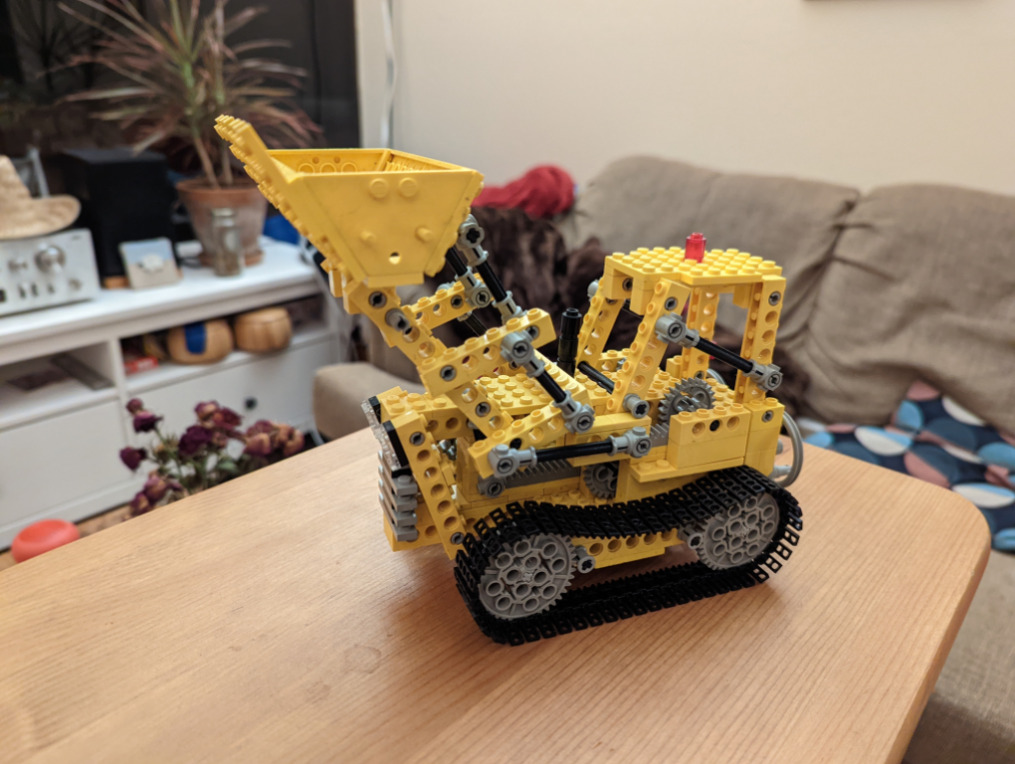
\includegraphics[width=\linewidth]{figures/pcas/lego.jpg} 
        \caption{RGB image}
    \end{subfigure}
    \begin{subfigure}{.32\linewidth}
        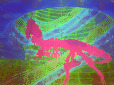
\includegraphics[width=\linewidth]{figures/pcas/trex_pca_sv.jpg}
        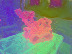
\includegraphics[width=\linewidth]{figures/pcas/lego_pca_sv.jpg} 
        \caption{Single-view PCA}
    \end{subfigure}
    \begin{subfigure}{.32\linewidth}
        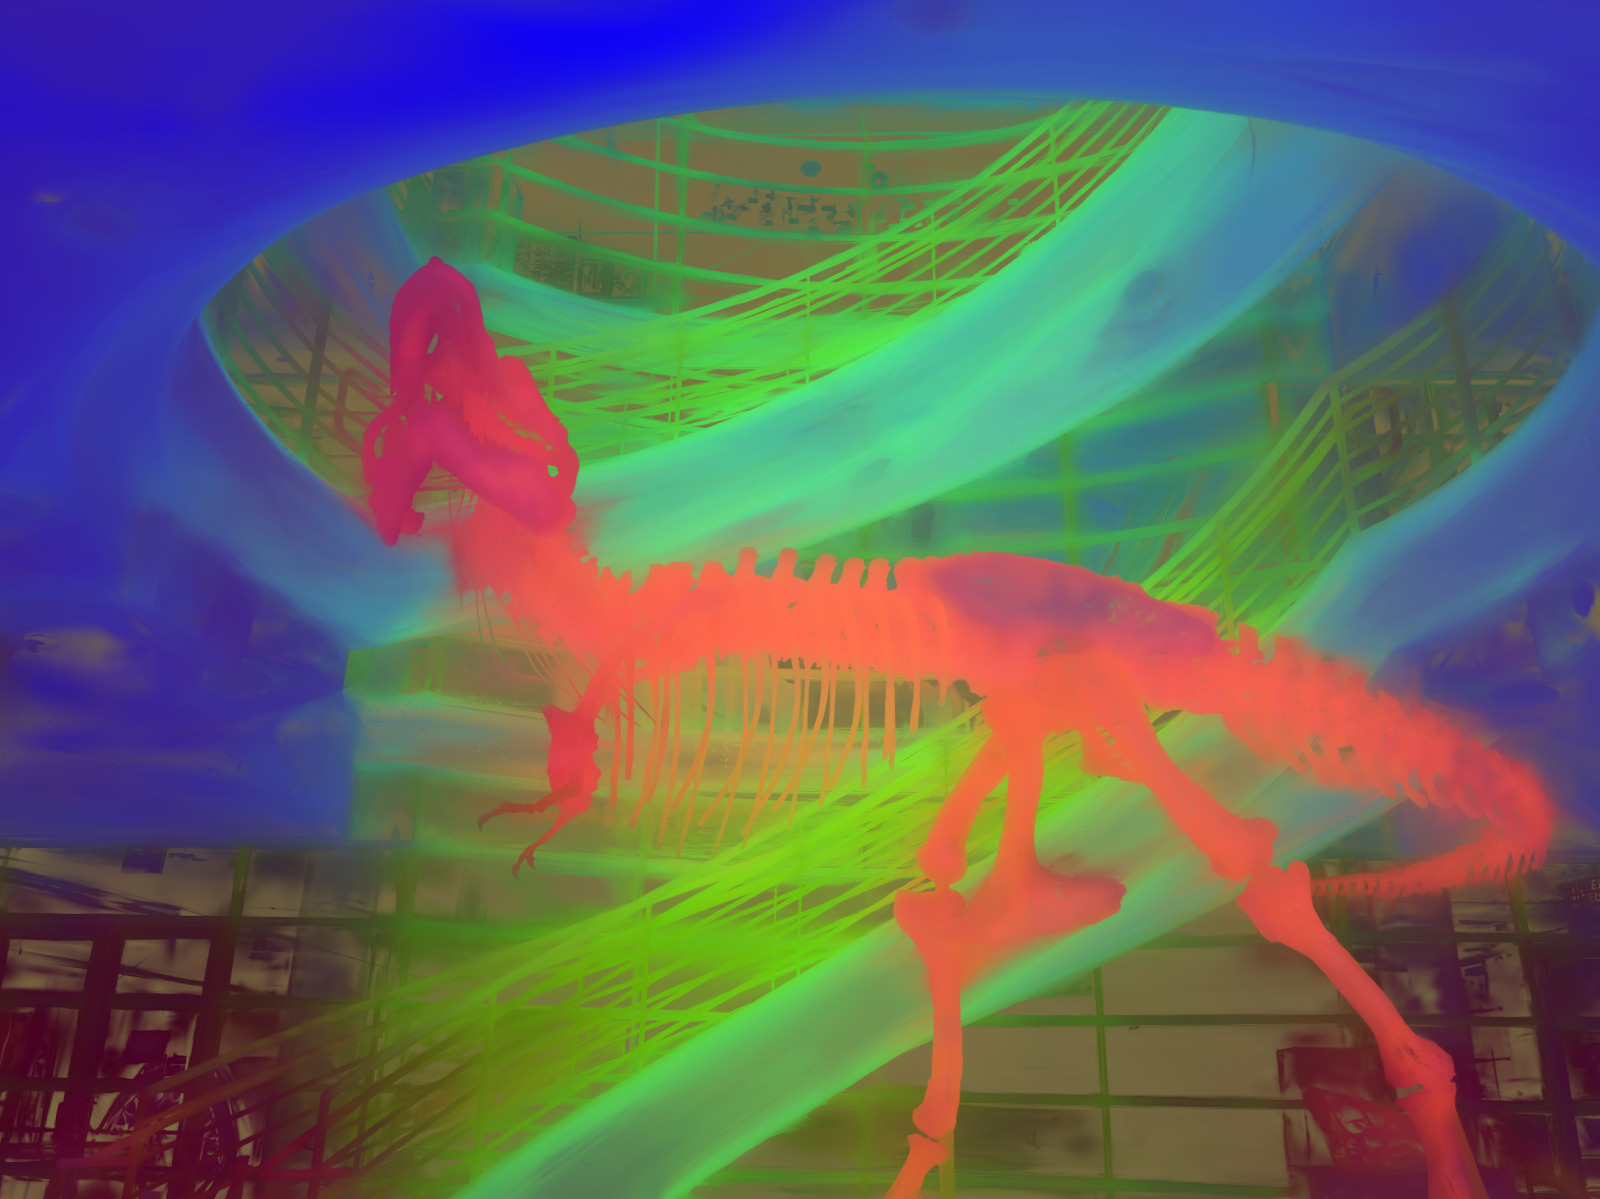
\includegraphics[width=\linewidth]{figures/pcas/trex_pca.jpg}
        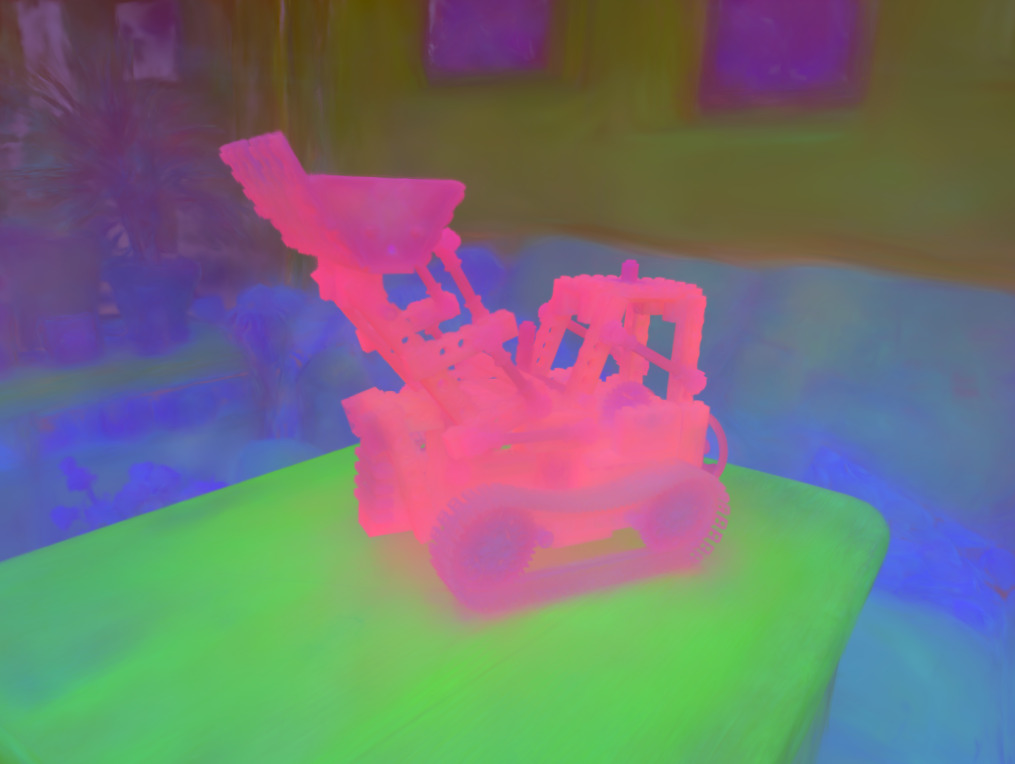
\includegraphics[width=\linewidth]{figures/pcas/lego_pca.jpg} 
        \caption{Multi-view PCA}
    \end{subfigure}
    \caption{\textbf{PCA visualizations.} The DINOv2 patch-level representations (middle) predicted from the RGB images (left) are aggregated into highly detailed 3D representations (right) using Eq.~(\ref{eq:uplifting}).}
    \label{fig:pca}
\end{figure}


\begin{figure}[t!]
    \centering
    \begin{subfigure}{.24\linewidth}
    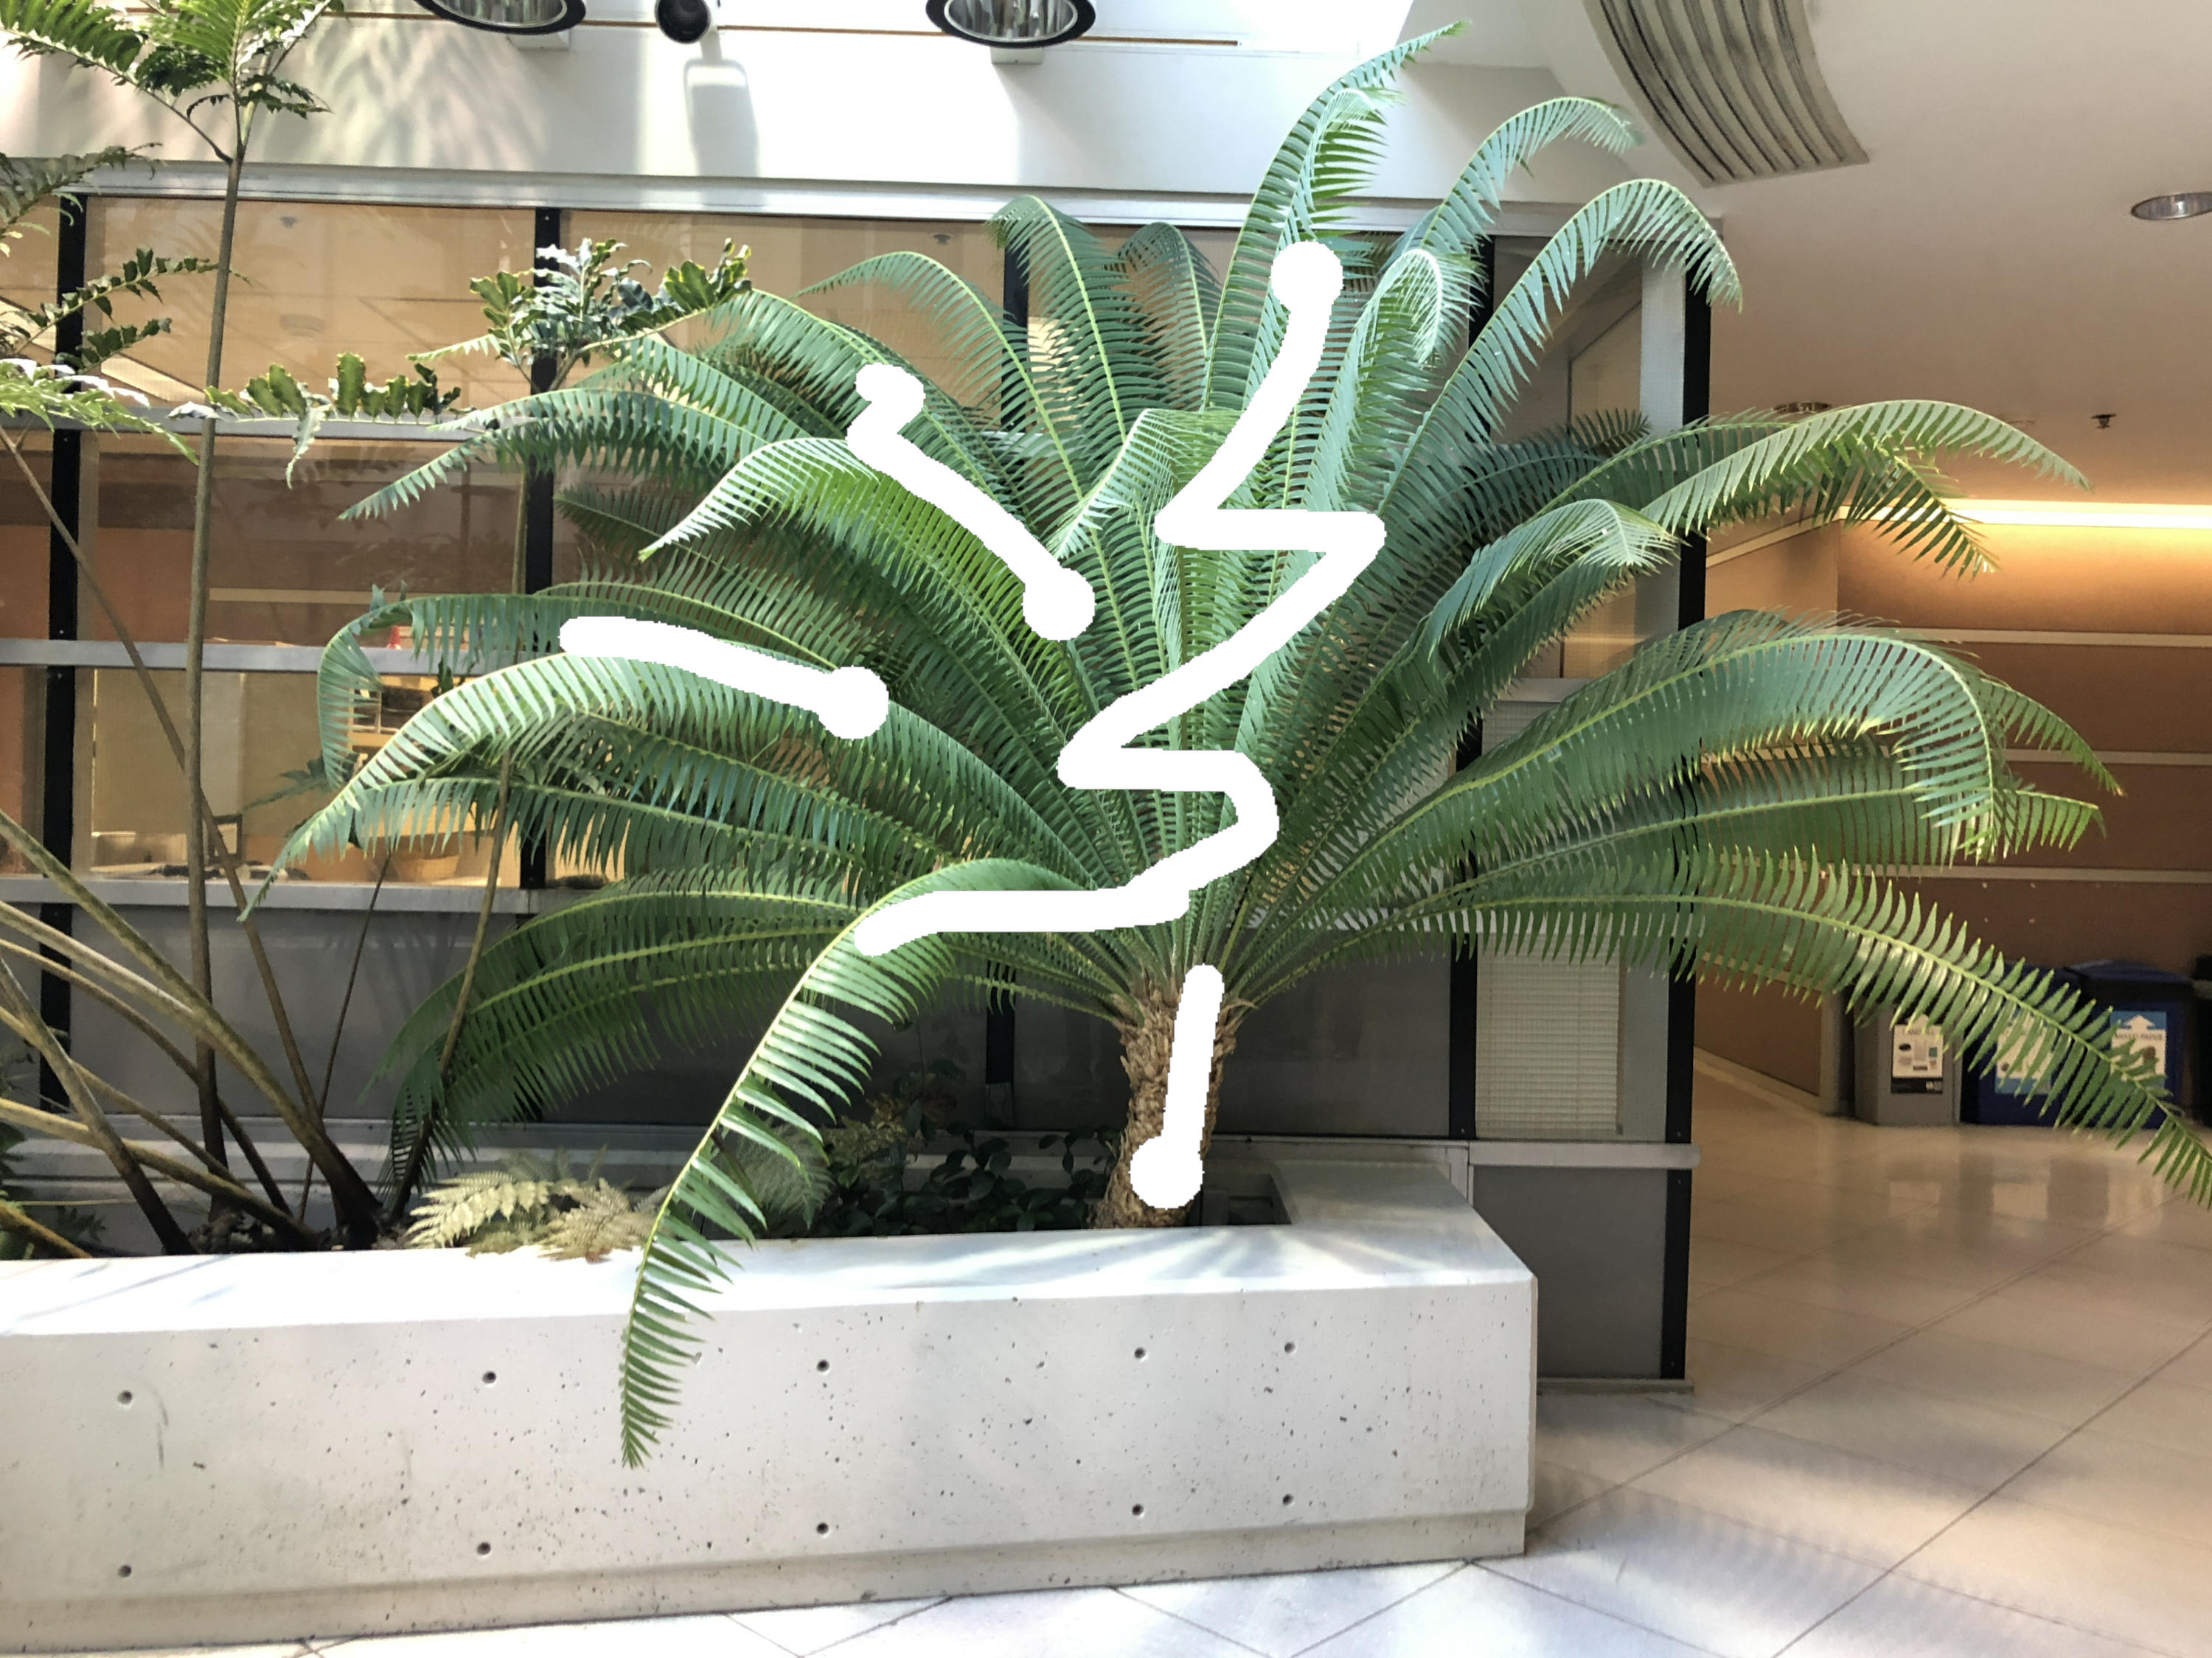
\includegraphics[width=\linewidth]{figures/diffusion/fern_rgb_pos.jpg}
    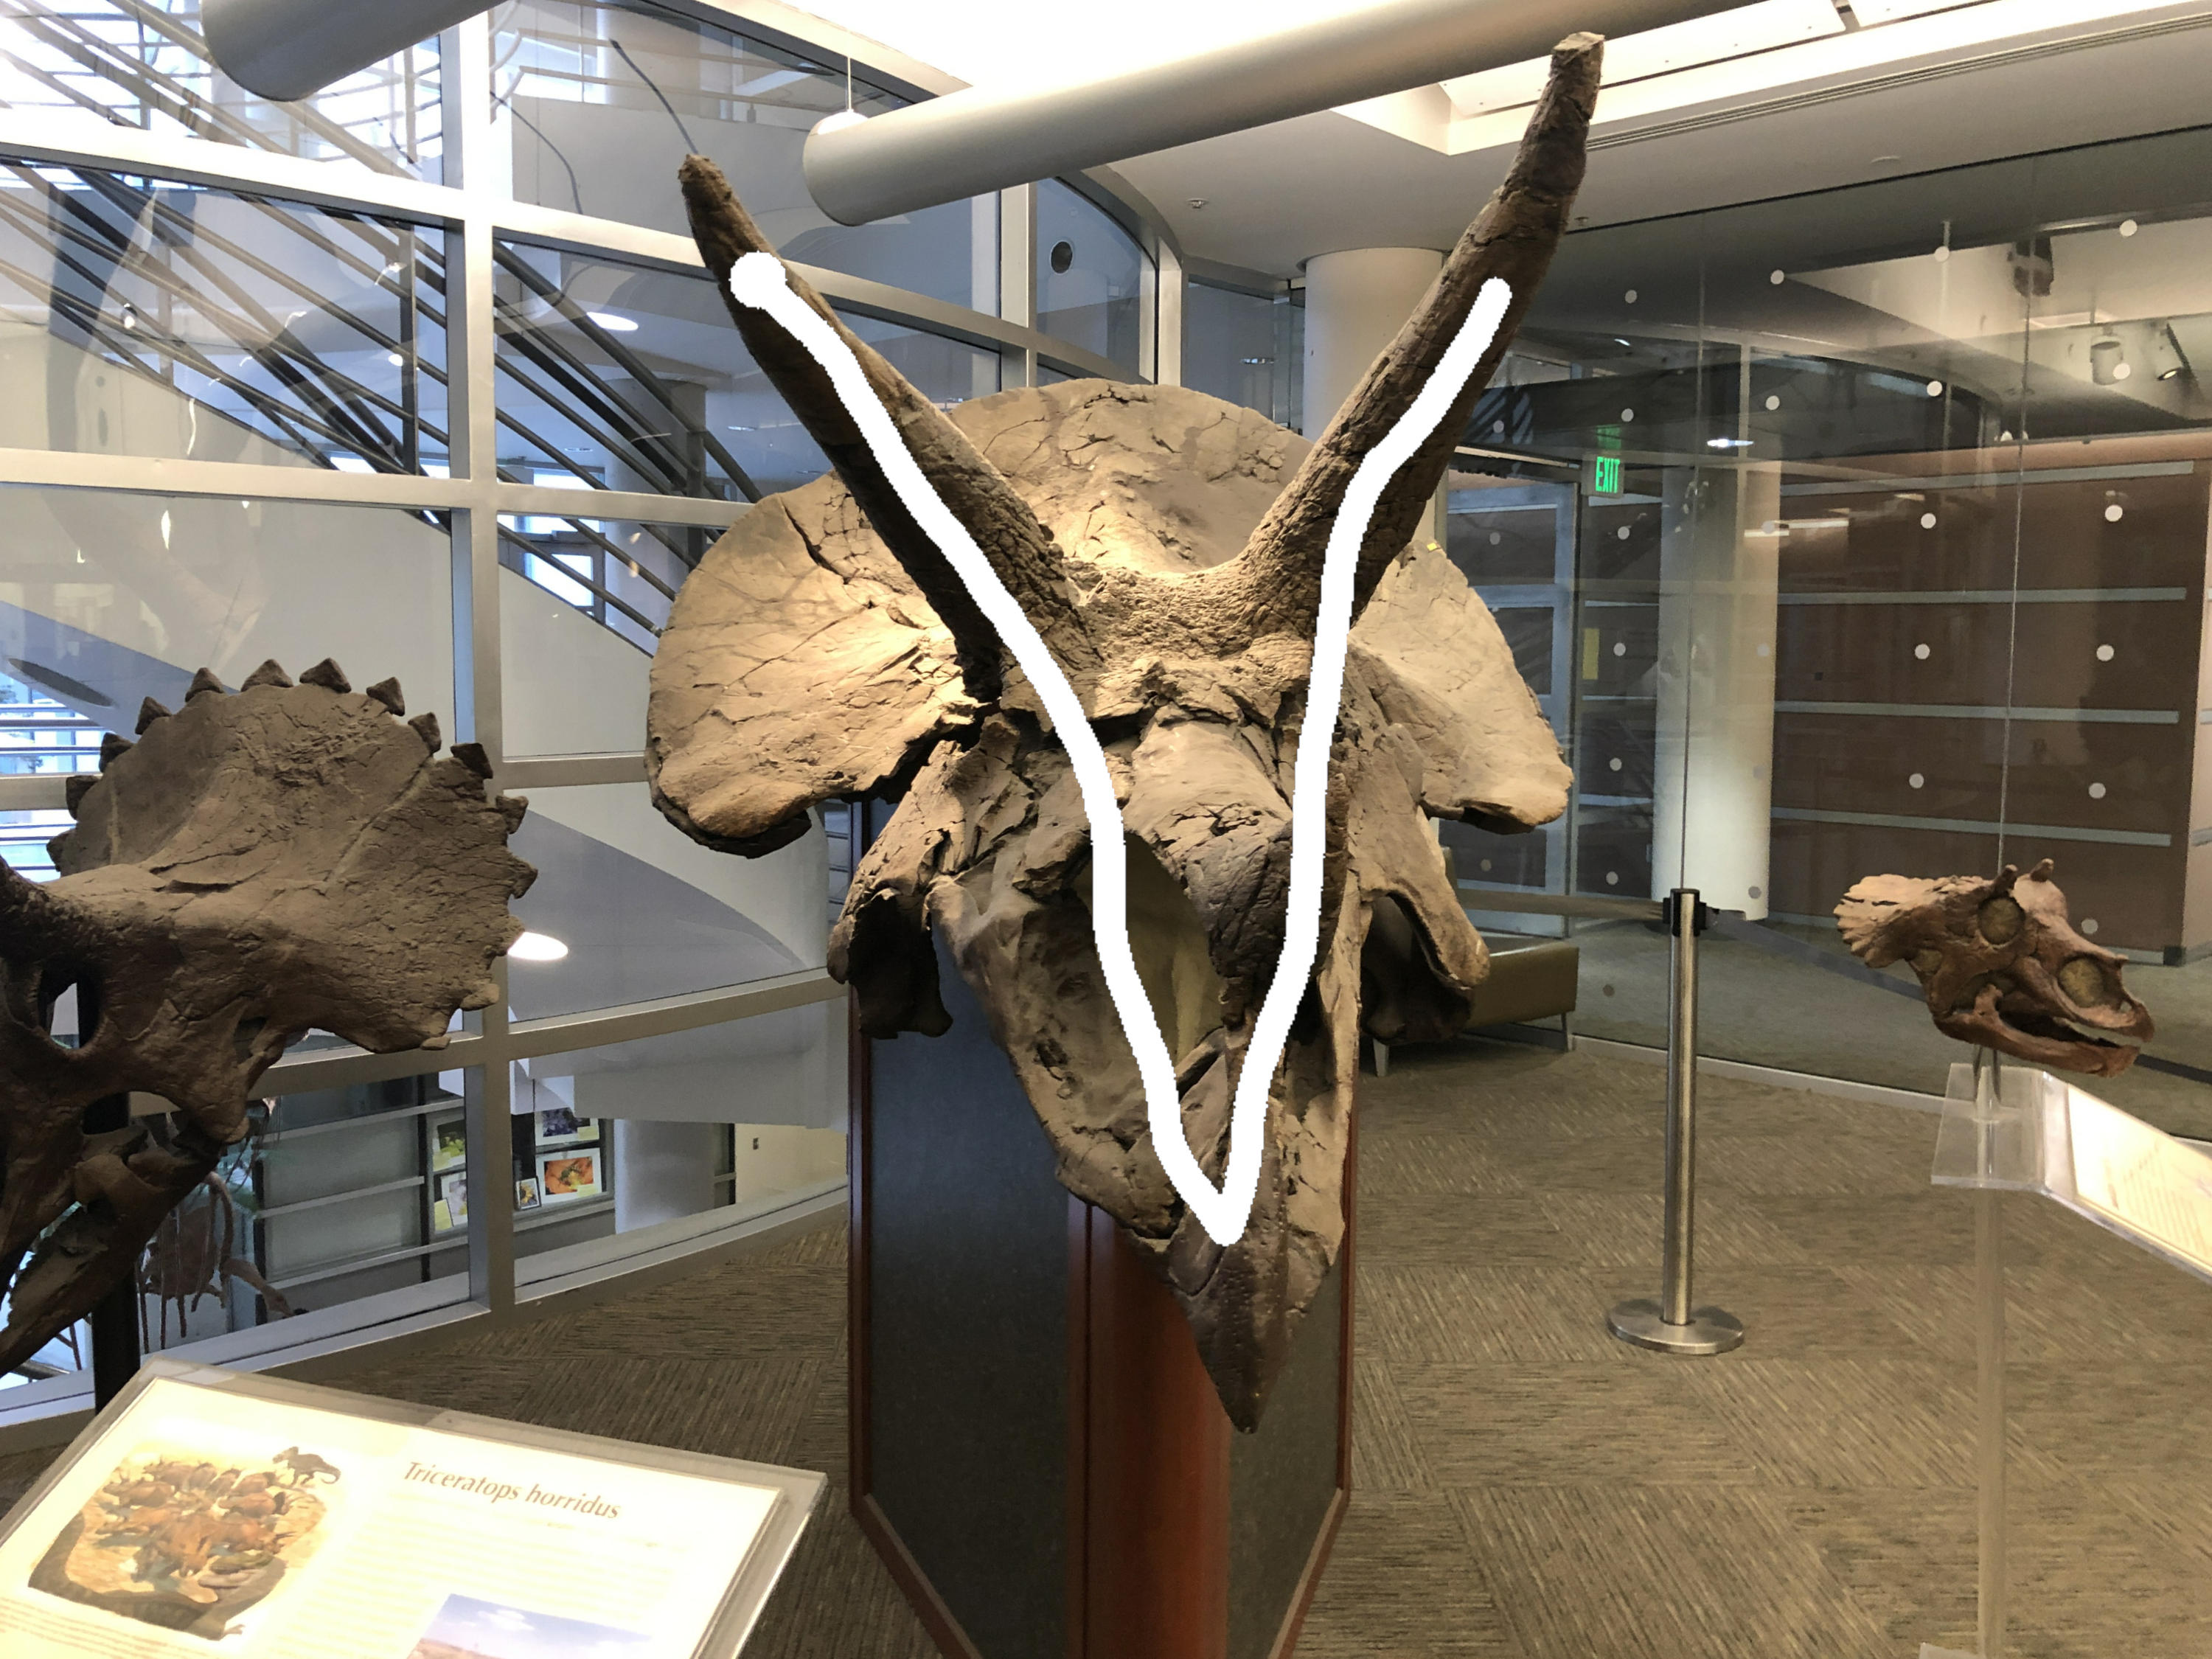
\includegraphics[width=\linewidth]{figures/diffusion/horns_rgb_pos.jpg}
    \subcaption{RGB image}
    \end{subfigure}
    \begin{subfigure}{.24\linewidth}
    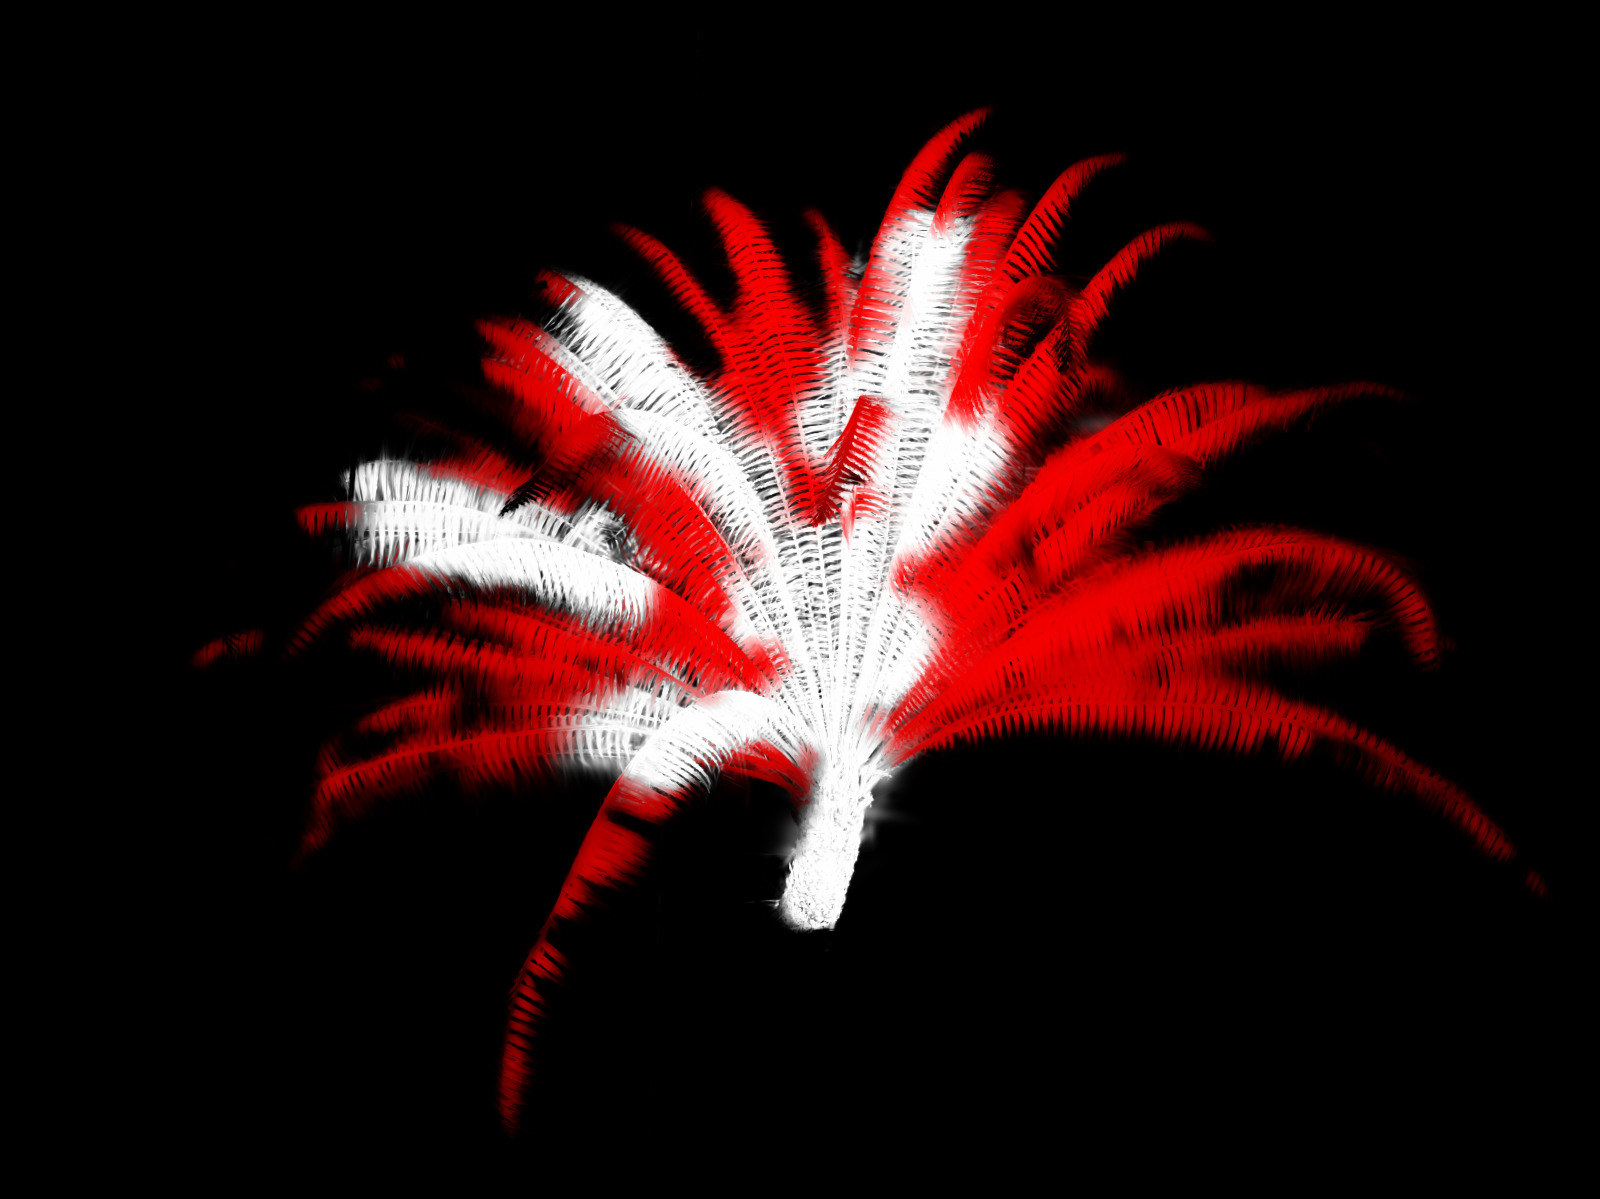
\includegraphics[width=\linewidth]{figures/diffusion/fern_sim3itreg.jpg} 
    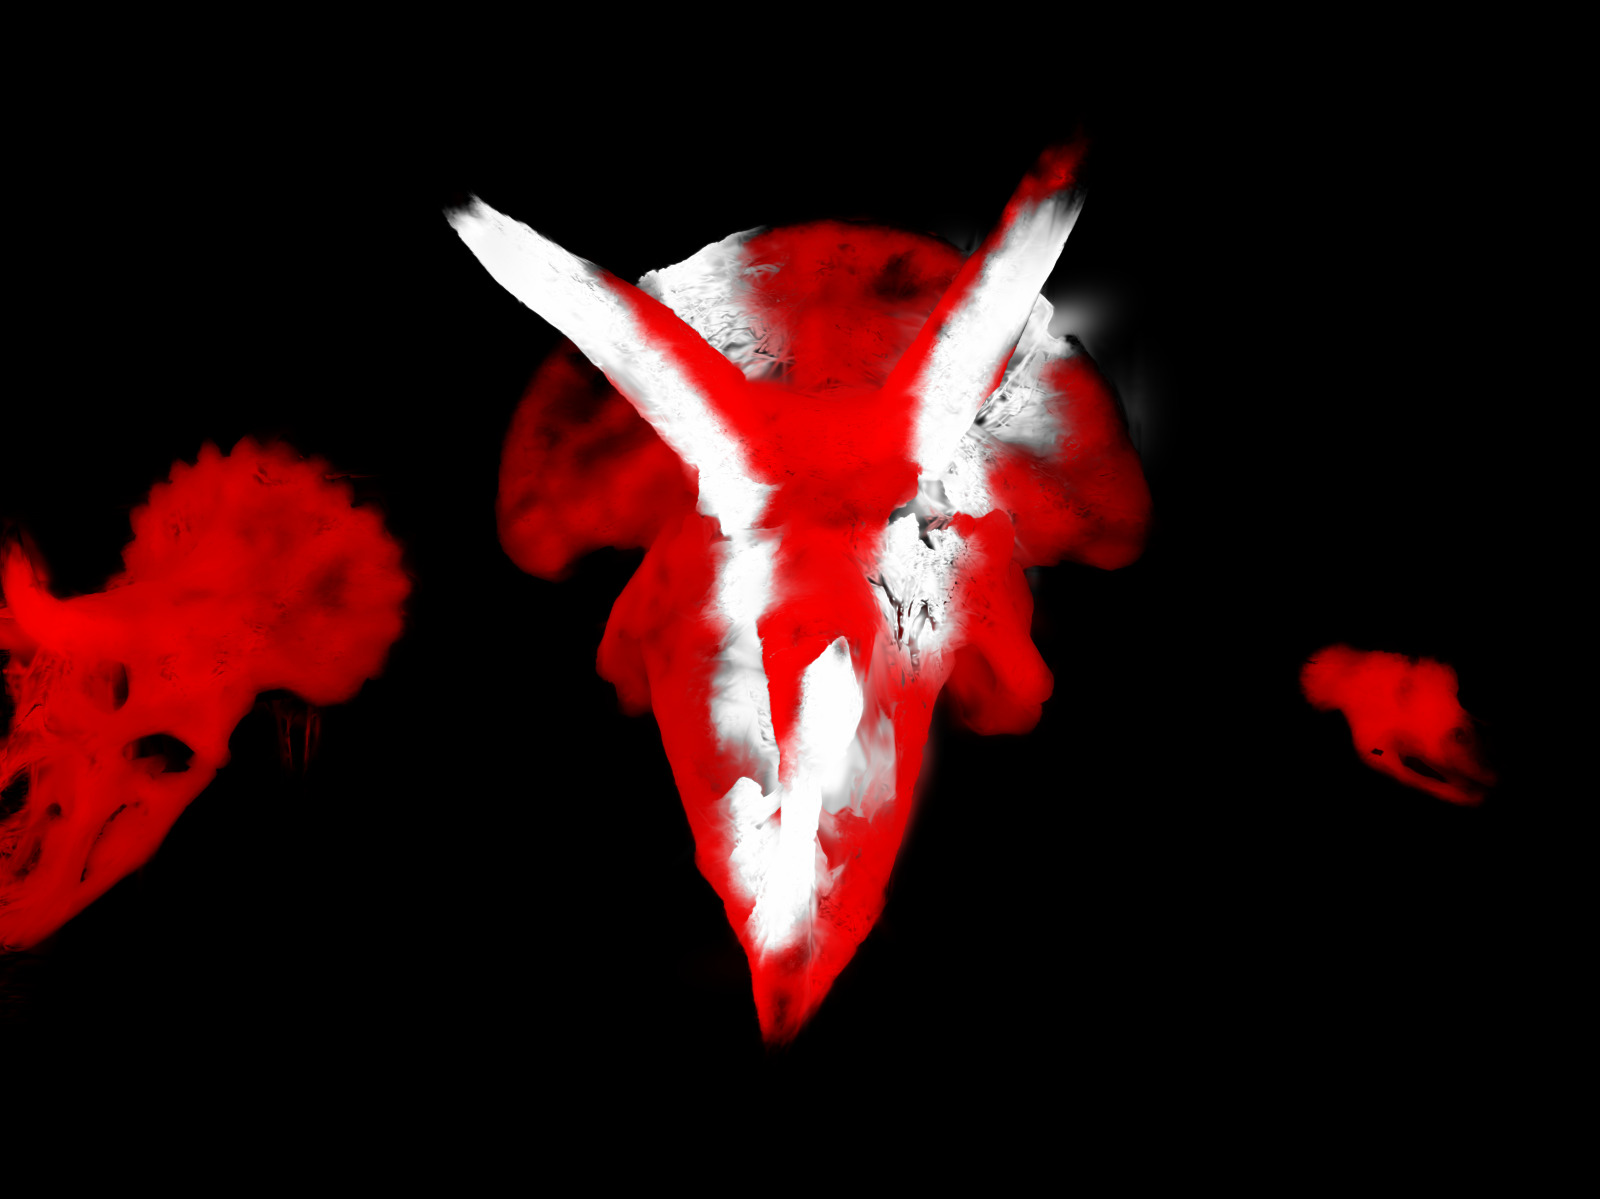
\includegraphics[width=\linewidth]{figures/diffusion/horns_sim3itreg.jpg}
    \caption{3 steps}
    \end{subfigure}
    \begin{subfigure}{.24\linewidth}
    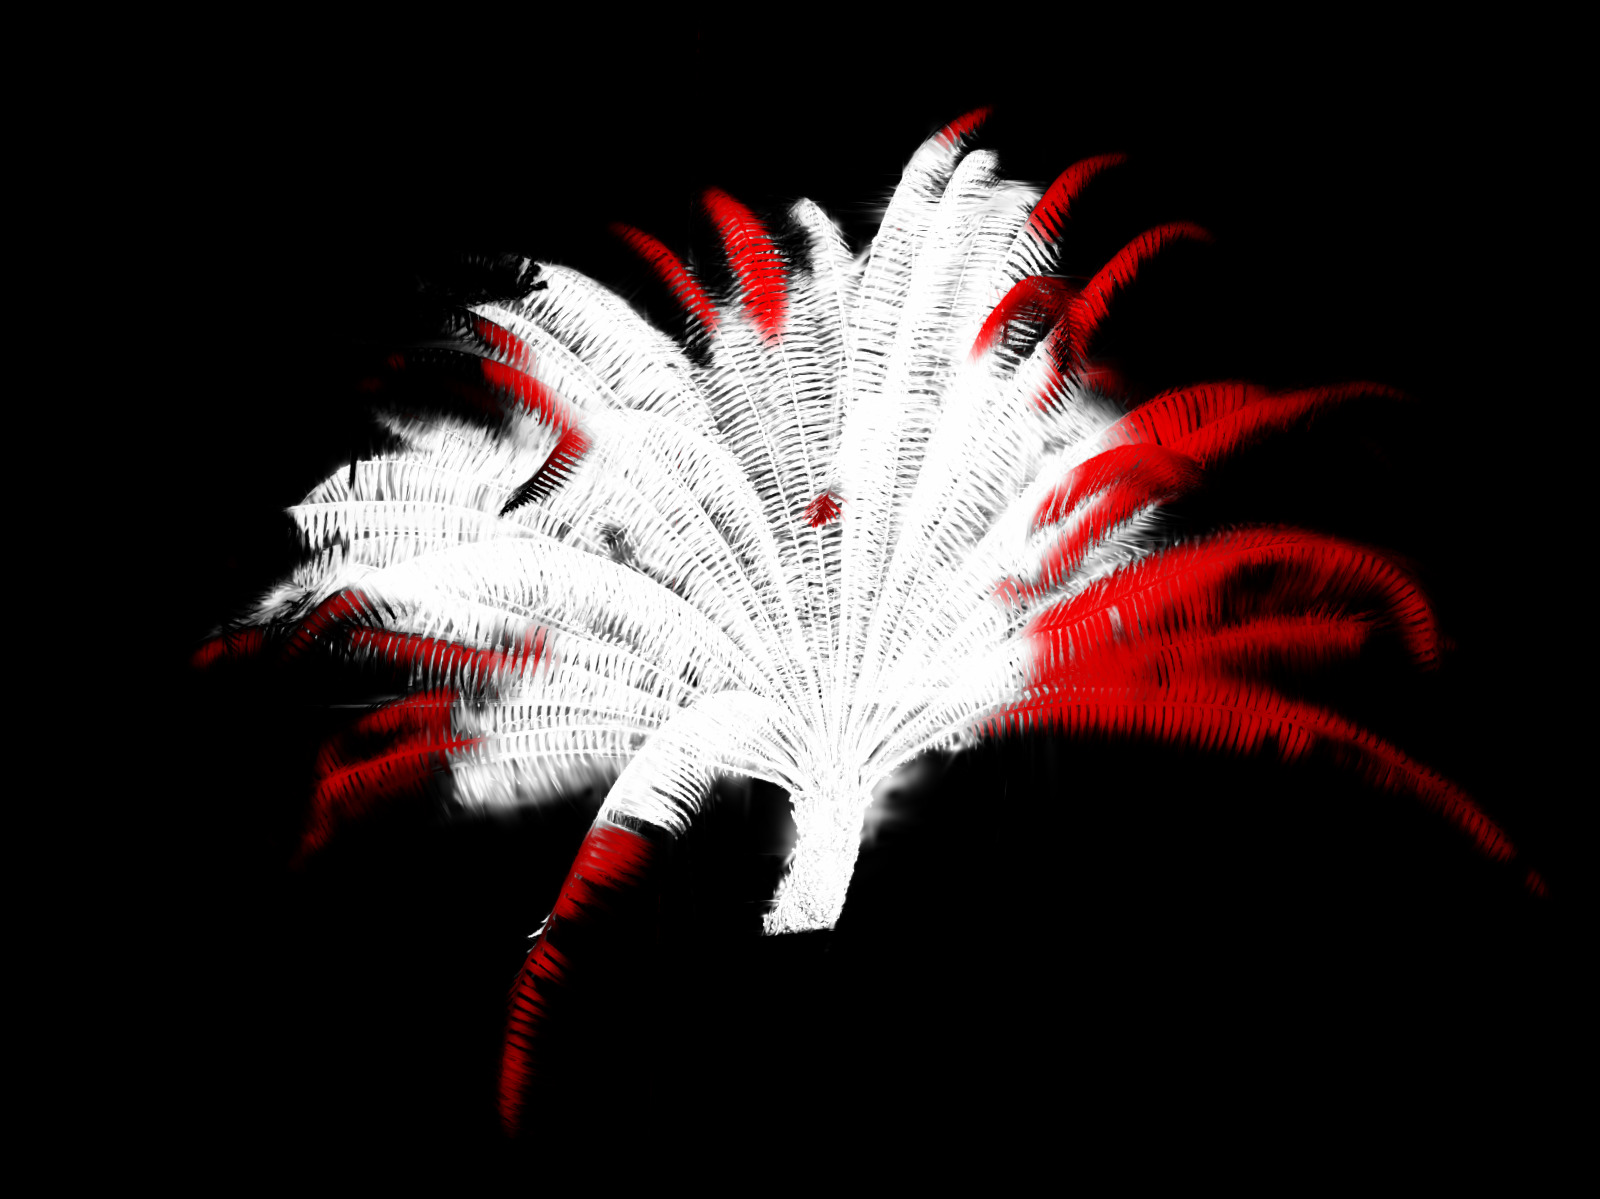
\includegraphics[width=\linewidth]{figures/diffusion/fern_sim7itreg.jpg}
    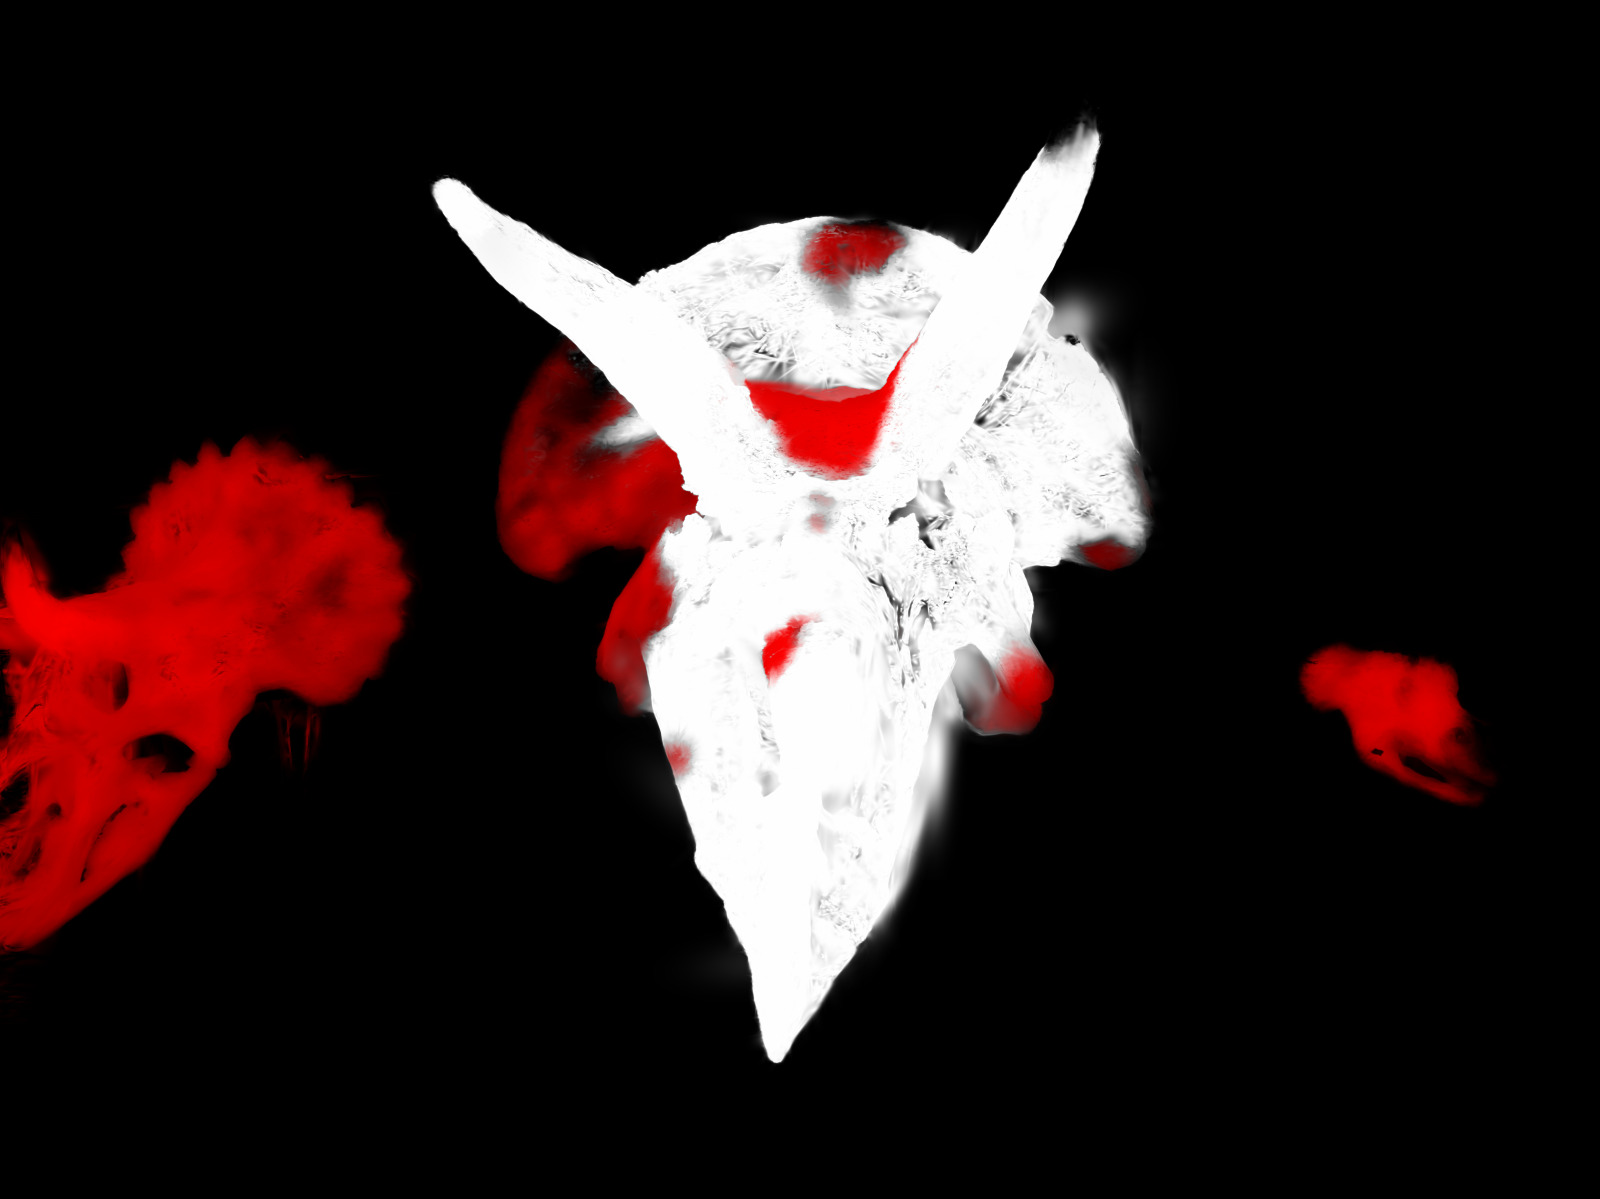
\includegraphics[width=\linewidth]{figures/diffusion/horns_sim7itreg.jpg}
    \subcaption{7 steps}
    \end{subfigure}
    \begin{subfigure}{.24\linewidth}
    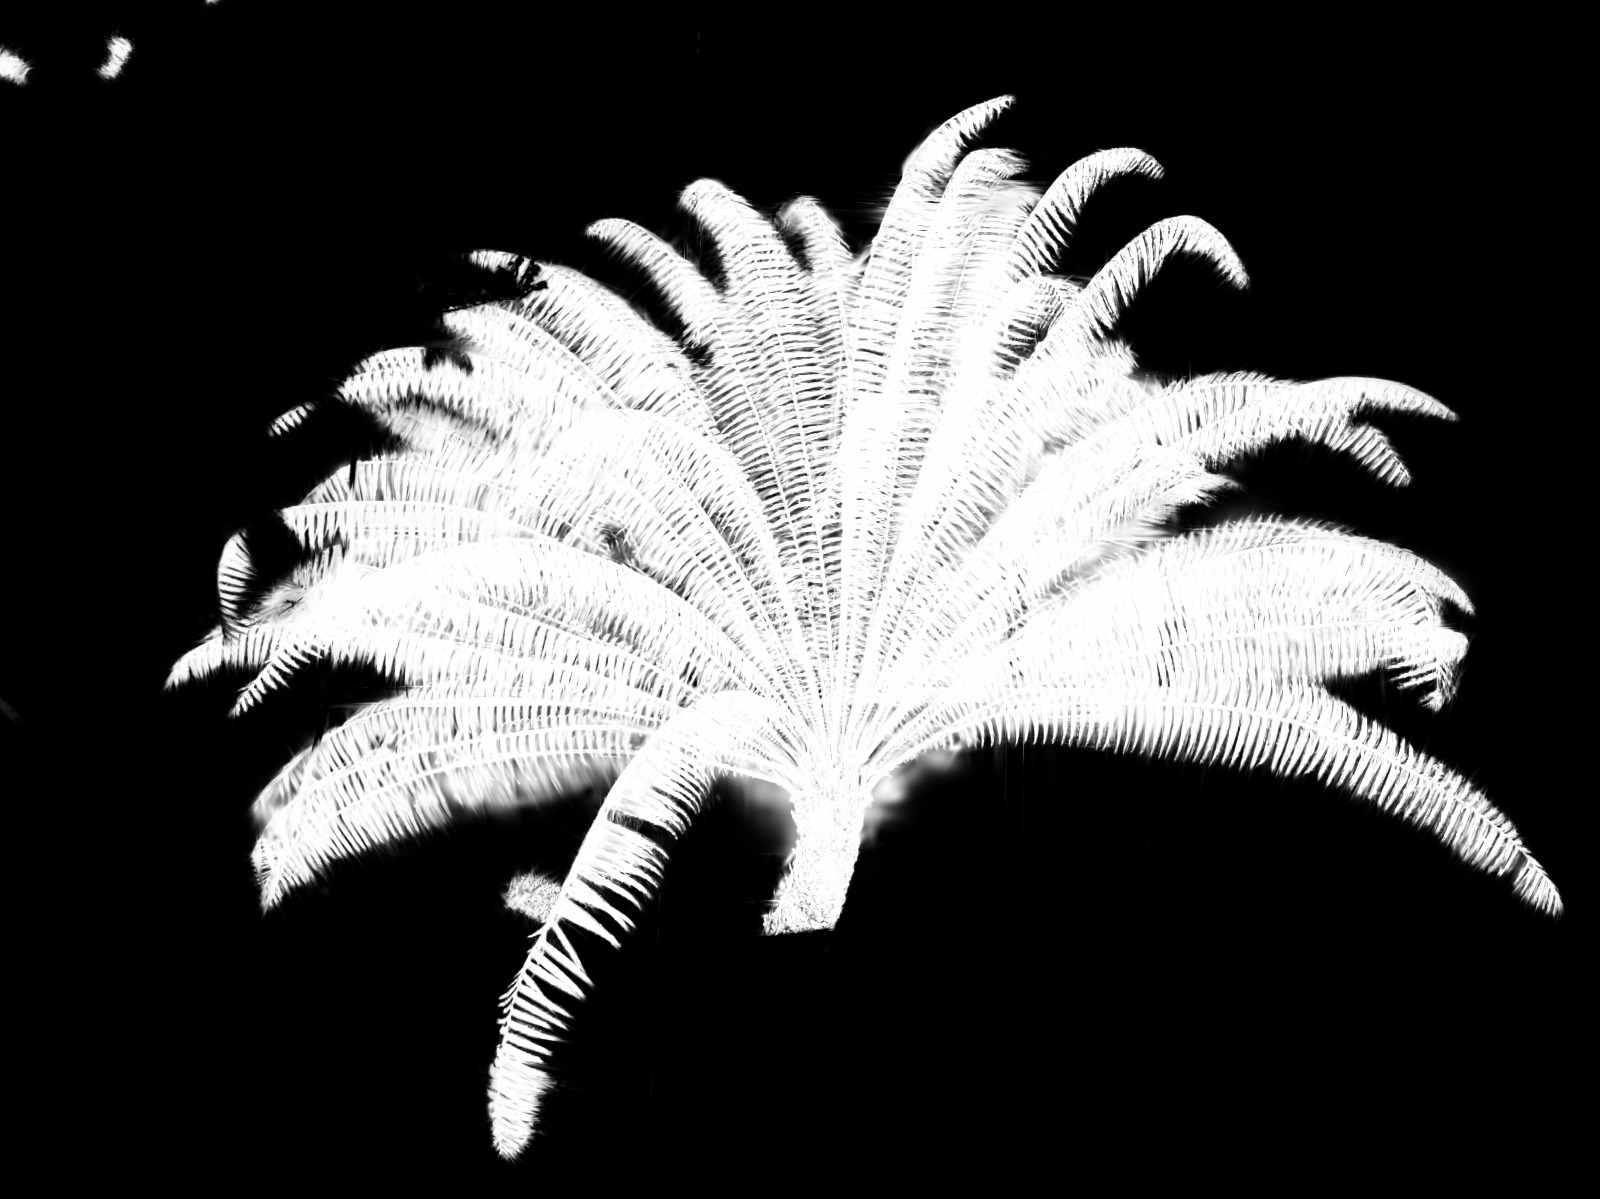
\includegraphics[width=\linewidth]{figures/diffusion/fern_simreg.jpg} 
    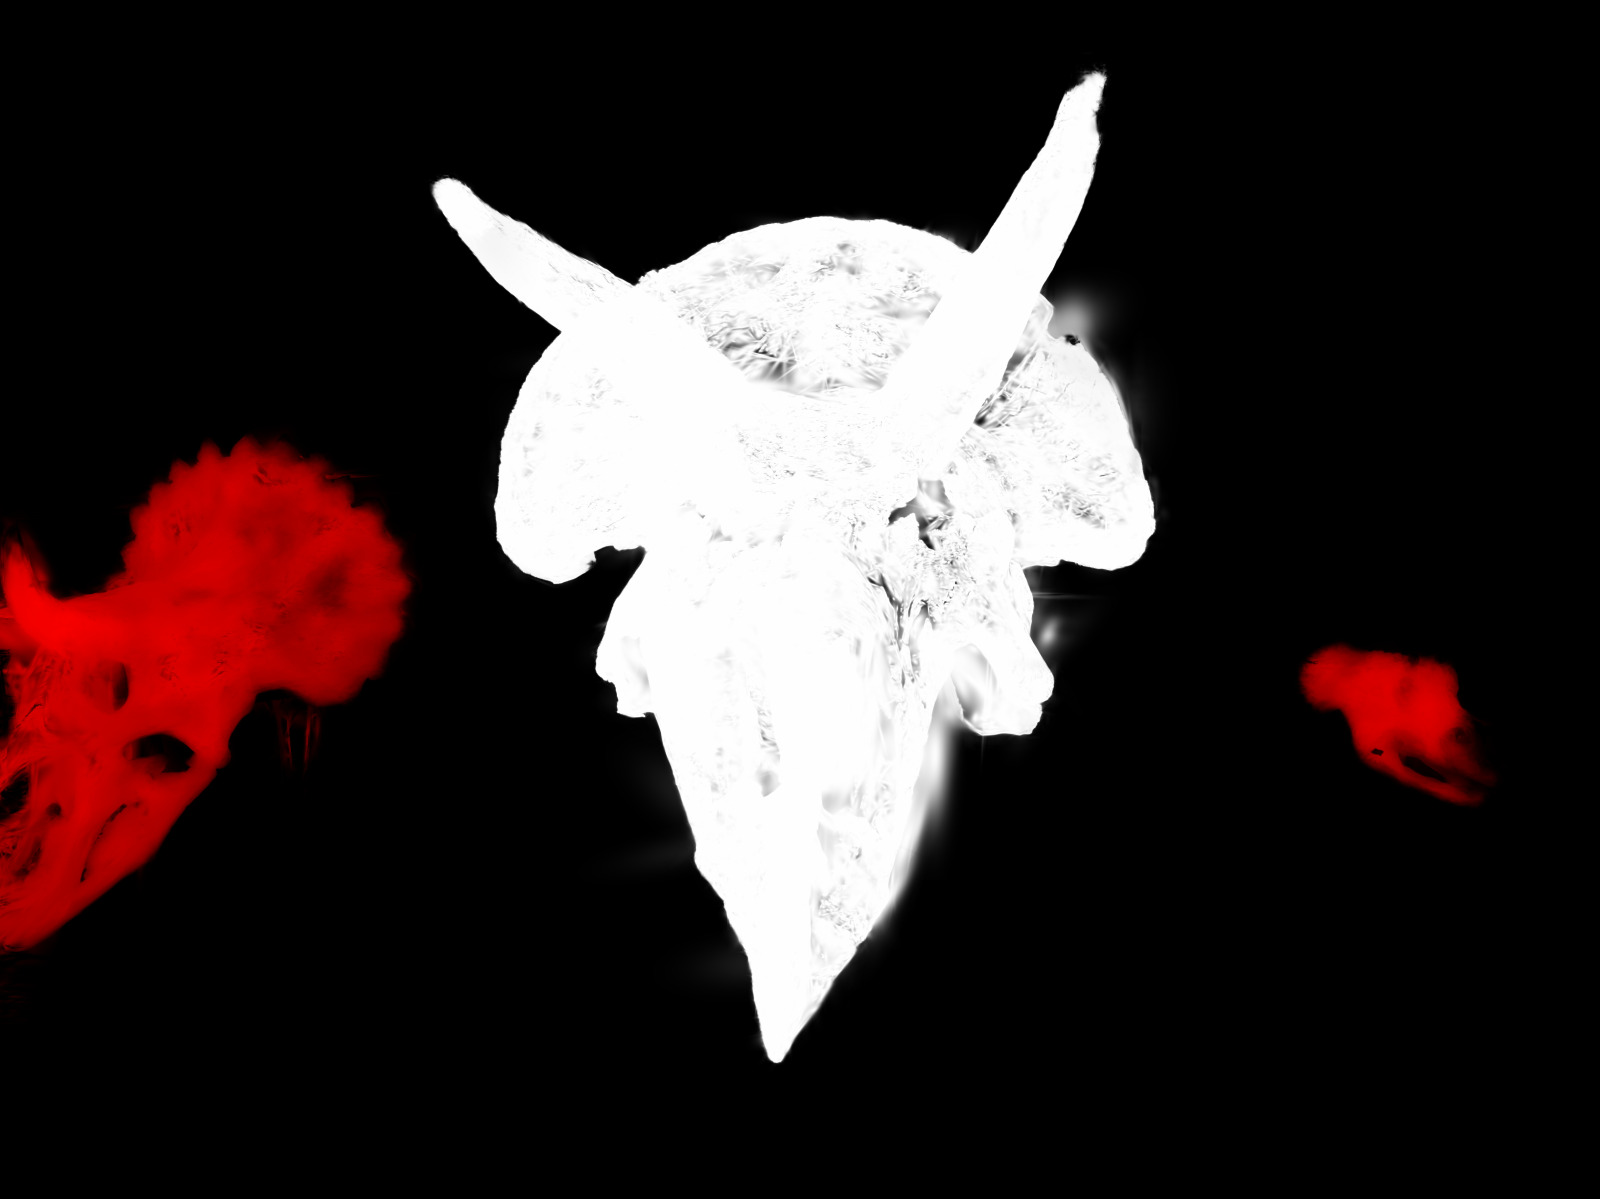
\includegraphics[width=\linewidth]{figures/diffusion/horns_simreg.jpg}
    \caption{100 steps}
    \end{subfigure}
    \caption{\textbf{Diffusion process.} 2D projection of the weight vector $g_t$ (white) and unary regularization term (red) at diffusion steps $t$. The diffusion process filters out unwanted objects that have similar features to the object of interest (such as the two smaller skulls on \emph{horns}, bottom-row), but are disconnected in space. The regularization term (red background) prevents leakage from the object to the rest of the scene (such as through the \emph{fern}'s trunk, top-row).}
    \vspace{-.1cm}
    \label{fig:diffusion}
\end{figure}

\begin{figure}[t]
    \centering
    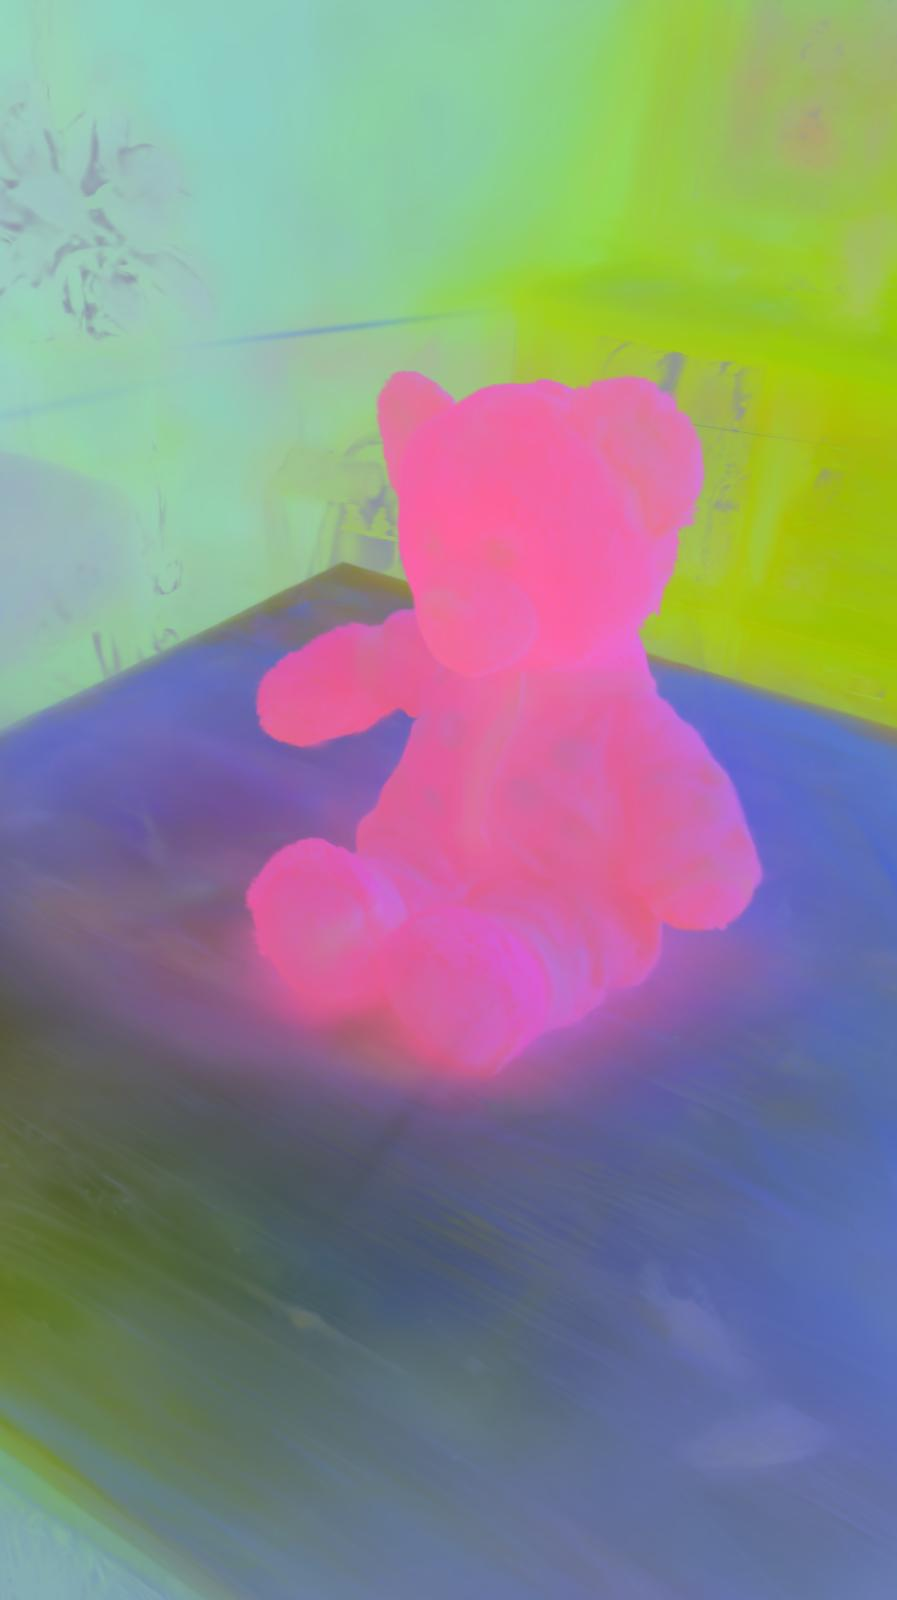
\includegraphics[width=0.32\linewidth, trim=0 500 0 200, clip]{figures/removal/pca.jpg}
    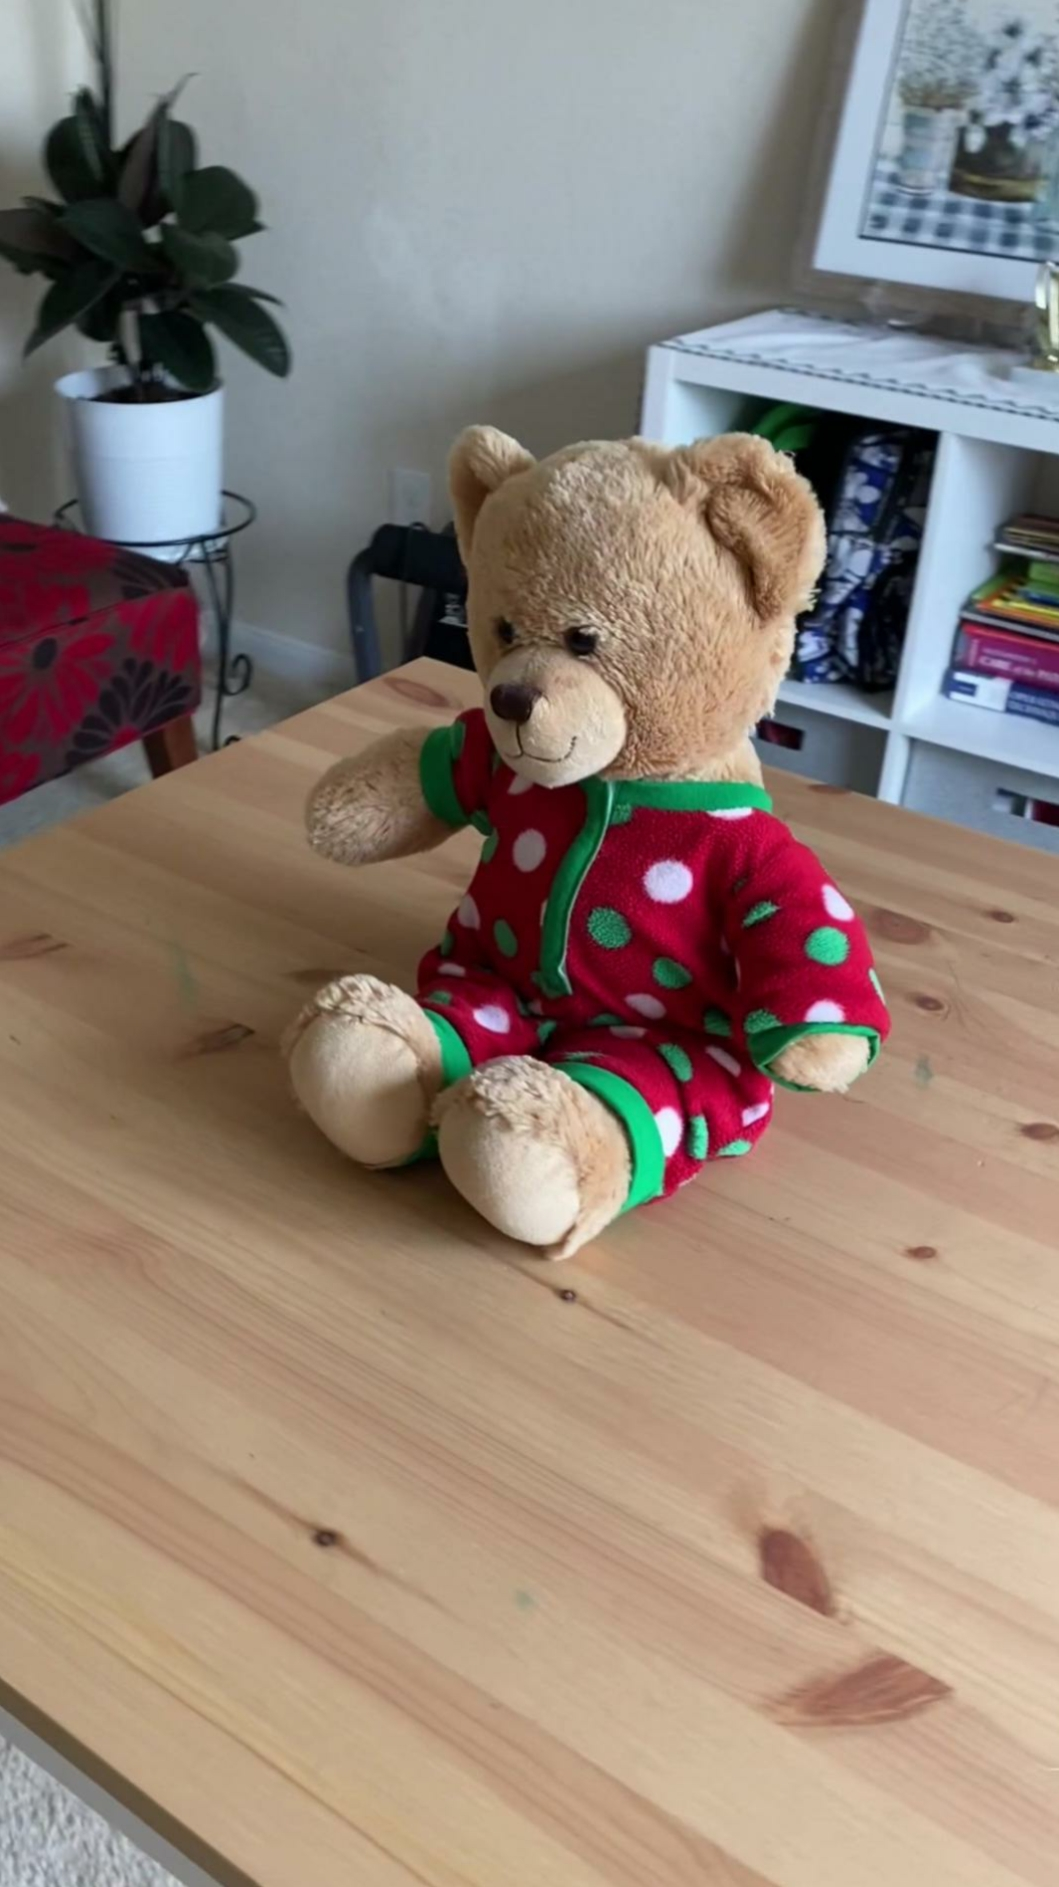
\includegraphics[width=0.32\linewidth, trim=0 610 0 200, clip]{figures/removal/img.jpg}
    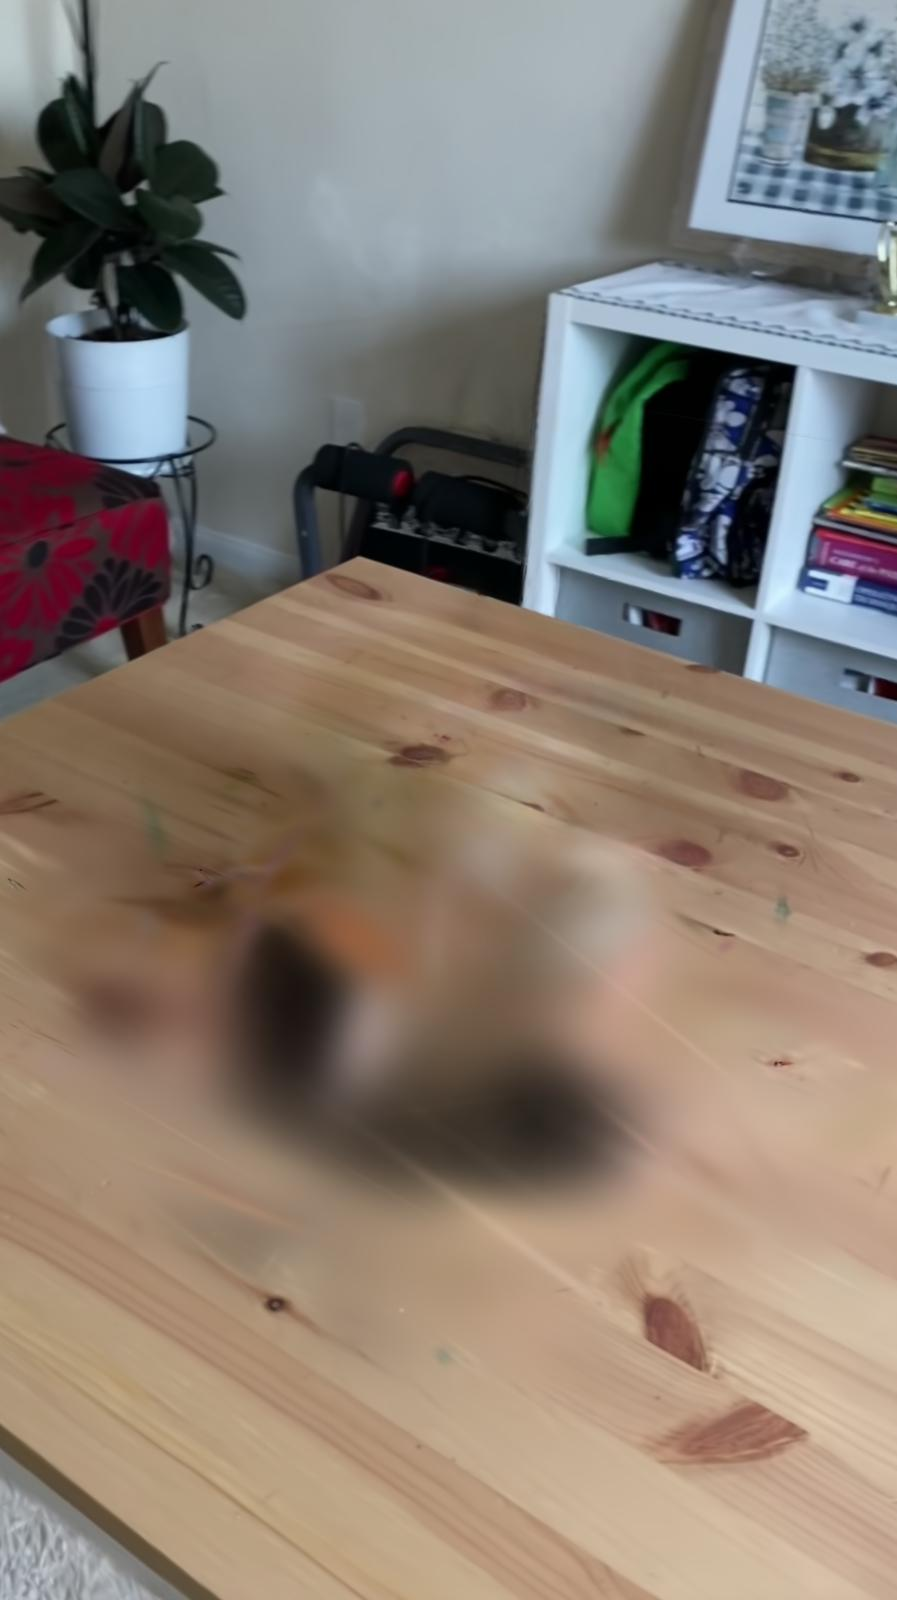
\includegraphics[width=0.32\linewidth, trim=0 500 0 200, clip]{figures/removal/removal-bis.jpg}
    \caption{\textbf{Open-vocabulary object removal.} Removing the teddy bear from the CO3D dataset~\citep{reizenstein2021co3d}, using DINOv2-guided graph diffusion based on 3D CLIP relevancy scores.}
    \vspace{-.3cm}
    \label{fig:removal-bonsai}
\end{figure}


\subsection{Multi-view segmentation results}
\label{sec:exp-seg}

\myparagraph{Task} In this section, we consider two segmentation tasks: (i)~Neural Volumetric Object Selection (NVOS)~\cite{ren2022nvos}, which is derived from the LLFF dataset~\citep{mildenhall2019llff}, and (ii)~SPIn-NeRF, which contains a subsets of scenes from NeRF-related datasets~\citep{knapitsch2017tanks, mildenhall2019llff, mildenhall2021nerf, yen2022nerfsupervision, fridovich2022plenoxels}.
%
NVOS consists of forward-facing sequences where the task is to predict the segmentation mask of a labeled frame based on reference scribbles from another frame. 
SPIn-NeRF contains both forward-facing and 360-degree scenes, in which all frames are labeled with segmentation masks, and the standard evaluation protocol uses the segmentation mask from the first frame as reference to label the subsequent frames.

\myparagraph{Setup}
We evaluate segmentation based on SAM and SAM2 mask uplifting and on DINOv2 feature uplifting combined with graph diffusion (see Sec.~\ref{sec:method_seg}). 
%
We compare our segmentation results (IoU) to the current state of the art: SA3D~\citep{cen2023segmentNeRF}, SA3D-GS~\citep{cen2023segmentGS}, SAGA~\citep{cen2023saga}, OmniSeg3D~\citep{ying2023omniseg3d}. All these methods are specifically designed for uplifting the 2D segmentation masks produced by SAM into 3D using gradient-based optimization of a projection loss. We also report results from NVOS \citep{ren2022nvos} and MVSeg \citep{yen2022nerfsupervision}, who respectively introduced the NVOS and SPIn-NeRF datasets.

\myparagraph{Results} Table~\ref{tab:nvos-spin} reports the average IoU across all scenes for NVOS and SPIn-NeRF. Per-scene results can be found in supplementary Tables \ref{tab:spin} and \ref{tab:nvos}.
Our results are comparable to the state of the art, while not relying on gradient-based optimization. 
Surprisingly, our segmentation with DINOv2 using graph diffusion also gives results on par with models leveraging SAM masks. Compared to SAM, DINOv2 better captures complex objects but sometimes also captures background noise. This can be seen in supplementary Fig.~\ref{fig:appendix-nvos}, T-Rex example: while SAM misses the end of the tail and ribs, DINOv2 captures the whole T-Rex but also includes part of the stairs behind.
Our lower segmentation results compared to OmniSeg's can partly be attributed to the poor Gaussian Splatting reconstruction of highly specular scenes, such as Fork. As also noted by \cite{cen2023saga}, the reconstruction includes semi-transparent Gaussians floating over the object, attempting to represent reflections or surface effects, which are challenging to capture using standard rasterization techniques~\citep{jiang2024gaussianshader}.


\myparagraph{Ablation study}
We compare our segmentation protocol using DINOv2 and SAM2 to multiple simpler variants. More precisely, we evaluate (i) a purely geometrical variant that reprojects the reference mask on the other views, without using SAM2 or DINOv2, (ii) single-view segmentation in 2D based on SAM2 or DINOv2 2D predictions, (iii) uplifting DINOv2 features or SAM2 masks into 3D then rendering them for segmentation, and (iv) segmenting using graph diffusion over DINOv2 3D feature similarities. Results are reported in Table~\ref{tab:ablation-spin-small}, and per-scene IoU as well as a detailed analysis can be found in supplementary Table~\ref{tab:ablation-spin-dino-sam} and Sec.~\ref{sec:appendix-seg_scene}. We observe that the purely geometrical approach works well on the forward-facing scenes and fails on 360-degree scenes. The single-view variant performs reasonably well on average, but the low resolution of patch-level representations (illustrated in  Fig.~\ref{fig:pca}) lead to a coarser segmentation. 3D uplifting considerably boosts results compared to single-view approaches, and introducing 3D spatial information through 3D graph diffusion further enhances results on the more challenging 360-degree scenes.

\begin{table*}[t!]
  \centering
  \footnotesize
\scalebox{0.9}{
\begin{tabular}{lccccccccc}
\toprule
& NVOS~\citep{ren2022nvos} & MVSeg~\citep{mirzaei2023spin} & SA3D-TRF~\citep{cen2023segmentNeRF} & SA3D-GS~\citep{cen2023segmentGS} & SAGA~\citep{cen2023saga} & OmniSeg3D~\citep{ying2023omniseg3d} & \multicolumn{3}{c}{\textbf{LUDVIG (Ours)}} \\
\cmidrule(lr){8-10}
3D representation &  &  & TensoRF & 3D-GS & 3D-GS & NeRF &  \multicolumn{3}{c}{3D-GS} \\
Uplifting & & & SAM & SAM & SAM & SAM &  DINOv2 & SAM & SAM2 \\
\midrule
NVOS & 70.1 & - & 90.3 & 92.2 & \textbf{92.6} & 91.7 & 92.4 & 91.3 & 91.3 \\
SPIn-NeRF & - & 90.9 & 93.7 & 93.2 & 93.4 & \textbf{94.3} & 93.8 & 93.8 & 93.8 \\
\bottomrule
\end{tabular}
}
  \caption{\textbf{Multi-view segmentation (IoU) on NVOS~\citep{ren2022nvos} and SPIn-NeRF~\citep{mirzaei2023spin}.} 
  %We obtain results on par with prior approaches, most of which leverage SAM for segmentation.
  }
  \label{tab:nvos-spin}
\end{table*}

\begin{table}[t!] 
\centering \footnotesize 
\scalebox{.85}{
\begin{tabular}{cccccc} 
\toprule
Geometry only & \multicolumn{2}{c}{Single view} & \multicolumn{2}{c}{Uplifting} & \multicolumn{1}{c}{Uplifting + Dif.} \\
\cmidrule(lr){2-3} \cmidrule(lr){4-6}
Reference mask & DINOv2 & SAM2 & DINOv2 & SAM2 & DINOv2 \\ 
\midrule
73.1 & 88.5 & 88.6 & 91.6 & 93.8 & 93.8 \\
\bottomrule 
\end{tabular} 
}
\caption{\textbf{Ablation on SPIn-NeRF segmentation}. We compare purely geometrical reference mask reprojection and single-view prediction with our feature/mask uplifting and graph diffusion.} 
\label{tab:ablation-spin-small} 
\end{table}
\begin{table}[t!]
\centering
\scalebox{0.87}{
\footnotesize
\begin{tabular}{lccccc}
\toprule
& ramen & figurines & teatime & waldo & \textbf{overall} \\ 
\midrule
LERF~\citep{kerr2023lerf}      & 62.0 & 75.0 & 84.8 & 72.7 & 73.6 \\ 
LangSplat~\citep{qin2023langsplat} & 73.2 & 80.4 & 88.1 & \textbf{95.5} & 84.3 \\ 
\textbf{LUDVIG (ours)}    &  \textbf{78.9} & \textbf{80.4} & \textbf{94.9} & 90.9 & \textbf{86.3} \\ 
\bottomrule
\end{tabular}
}
\vspace{-.1cm}
\caption{\textbf{LERF object localization.} Comparison with the state of the art on the dataset introduced by LangSplat~\citep{qin2023langsplat}.}
\label{tab:lerf-loc}

\end{table}

\begin{table}[t!]
\centering
\scalebox{0.85}{
\footnotesize
\begin{tabular}{lcccccc}
\toprule
%\cmidrule(lr){3-7}
& \multirow{2}{*}{ramen} & \multirow{2}{*}{figurines} & \multirow{2}{*}{teatime} & \multirow{2}{*}{waldo} & \multirow{2}{*}{\textbf{overall}} & time \\
& &&&&& (min) \\ \midrule
\multicolumn{7}{l}{\emph{Initial evaluation protocol from~\cite{kerr2023lerf,qin2023langsplat}: 2D object segmentation}} \\
\midrule
LERF~\citep{kerr2023lerf}      & 28.2 & 38.6 & 45.0 & 37.9 & 37.4 & 45  \\ 
LangSplat~\citep{qin2023langsplat} & 51.2 & 44.7 & 65.1 & 44.5 & 51.4 & 105 \\ 
LUDVIG (ours)    & \textbf{58.1} & \textbf{63.3} & \textbf{77.1} & \textbf{58.5} & \textbf{64.3} & 10 \\ 
\midrule 
\multicolumn{7}{l}{\emph{New evaluation protocol introduced in OpenGaussian~\cite{wu2024opengaussian}: 3D object selection}} \\
\midrule
%OpenGaussian~\citep{wu2024opengaussian} & 31.0 & 39.3 & 60.4 & 22.7 & 38.4 & 50 \\ 
OpenGaussian~\citep{wu2024opengaussian} & 23.9 & 59.3 & 54.4 & 34.6 & 43.1 & 50 \\ 
Dr. Splat~\citep{jun2025drsplat} & 24.7 & 53.4 & 57.2 & 39.1 & 43.6 & - \\ 
LUDVIG (ours)   & \textbf{42.3} & \textbf{58.0} & \textbf{58.6} & \textbf{42.8} & \textbf{50.4} & 10 \\ 
\bottomrule
\end{tabular}
}
\caption{\textbf{LERF object segmentation.} 
We evaluate on the LERF dataset introduced by LangSplat~\citep{qin2023langsplat} with two different evaluation protocols: i) segmentation based on the 2D reprojected features, ii) 3D segmentation (or \emph{object selection} and reprojection of the \emph{binary 3D masks}, proposed by \cite{kerr2023lerf, qin2023langsplat} and \cite{wu2024opengaussian} respectively.}
\label{tab:lerf-seg}

\end{table}

\subsection{Open-vocabulary object localization}
\label{sec:exp-clip}

\myparagraph{Task}
We evaluate on the LERF dataset~\citep{kerr2023lerf}, which includes localization and segmentation tasks on complex in-the-wild scenes. We report our results on the extended evaluation task introduced by LangSplat~\citep{qin2023langsplat} containing additional challenging localization samples.



\myparagraph{Setup}
For localization, we simply reproject the 3D CLIP relevancy scores and follow the evaluation protocol from LangSplat~\citep{qin2023langsplat}. 
For segmentation, we consider two evaluation protocols:
(i) \textit{standard 2D segmentation}, as introduced by~\citep{kerr2023lerf} (top part of the table), and (ii) \emph{3D object selection}, which consists of binarizing the 3D masks before rendering (bottom part). The latter protocol was introduced in~\citep{jun2025drsplat} as a way to better assess the quality of 3D semantic features, such as 3D CLIP features, compared to prior existing protocols which focus on the performance on 2D downstream tasks.
For both approaches, we refine raw 3D CLIP relevancy scores using graph diffusion and use them for segmentation as follows. For
(i) we perform 2D segmentation from rendered features using SAM, as described in Sec.~\ref{sec:method_clip}, which we compare to 2D segmentation by LERF~\citep{kerr2023lerf} and LangSplat~\citep{qin2023langsplat} (top of table).
For (ii) we directly segment in 3D by binarizing the diffused features before rendering them, then computing 2D segmentation masks from these rendered features. We use automatic thresholding for binarization before and after rendering. 

\myparagraph{Results} 
Table~\ref{tab:lerf-loc} reports object localization results, where our method outperforms LangSplat despite not relying on SAM for this task.
Table~\ref{tab:lerf-seg} presents segmentation results along with average runtimes, which account for feature map generation and 3D feature training when applicable.
Across both evaluation settings, our method consistently surpasses prior approaches while achieving a 5 to 10$\times$ speedup in feature generation and uplifting.

\myparagraph{Runtime analysis}
Our approach based on graph diffusion offers fast feature map generation compared to leveraging SAM’s automatic mask generation in 2D as in \citep{qin2023langsplat,wu2024opengaussian}, but it comes with additional inference-time overhead. This tradeoff is further discussed in supplementary Sec.~\ref{sec:appendix-runtime-comp}. When inference time is a critical constraint, LUDVIG’s uplifting can also be applied directly to full segmentation masks, following the same setup as LangSplat~\citep{qin2023langsplat} and OpenGaussian~\citep{wu2024opengaussian}, as shown in the next section.

\begin{table}[t!]
\centering
\scalebox{0.88}{
\footnotesize
\begin{tabular}{cccccccc}
\toprule
%\cmidrule(lr){3-7} 
SAM & Graph diffusion & ramen & figurines & teatime & waldo & overall \\ 
\midrule
\xmark & \xmark  & 27.8 & 37.8 & 38.2 & 30.4 & 33.6 \\ 
\xmark & \cmark   & 42.3 & 58.0 & 58.6 & 42.9 & 50.4 \\ 
\cmark & \xmark  & 52.2 & 51.8 & 68.9 & 56.4 & 57.3 \\ 
\cmark & \cmark  & \textbf{58.1} & \textbf{63.3} & \textbf{77.1} & \textbf{58.5} & \textbf{64.3} \\ 
\bottomrule
\end{tabular}
}
\caption{\textbf{Ablation on LERF object segmentation.} Results (IoU) with and without using 3D graph diffusion and/or 2D SAM segmentation, evaluated on the dataset introduced by LangSplat~\citep{qin2023langsplat}.}
\label{tab:ablation-lerf}
\end{table}

\myparagraph{Ablation study}
%
Table~\ref{tab:ablation-lerf} presents an ablation study on the effect of graph diffusion and SAM-based segmentation following the first evaluation protocol (top part) in Table~\ref{tab:lerf-seg}. 

\subsection{Open-vocabulary semantic segmentation}
\label{sec:exp-semantic}

\myparagraph{Task}
We evaluate on ScanNetv2~\citep{dai2017scannet}, which provides posed RGB images from video scans, reconstructed point clouds, and ground-truth 3D point-level semantic labels.


\myparagraph{Setup}
We follow the evaluation protocol of OpenGaussian~\citep{wu2024opengaussian}.  
In particular, we train Gaussian Splatting by initializing from the ground-truth point cloud, keeping the 3D positions fixed and disabling densification.
For this task, we replace OpenGaussian’s quantized feature learning with our uplifting process, leaving the rest of the protocol unaltered. Specifically, we uplift 2D segmentation masks generated by SAM based on textual queries, as in the prior works we compare to \citep{qin2023langsplat,shi2024legaussians, wu2024opengaussian}.

\myparagraph{Results} 
As shown in Table~\ref{tab:scannet},
our approach yields significant accuracy gains over OpenGaussian~\citep{wu2024opengaussian}, while being considerably simpler and faster than their quantization-based learning process.
\begin{table}[t]
\centering
\footnotesize
\scalebox{.95}{
\begin{tabular}{lcccccc}
\toprule
\multirow{2}{*}{Methods} & \multicolumn{2}{c}{19 classes} & \multicolumn{2}{c}{15 classes} & \multicolumn{2}{c}{10 classes} \\
\cmidrule(lr){2-3} \cmidrule(lr){4-5} \cmidrule(lr){6-7}
 %& mIoU $\uparrow$ & mAcc. $\uparrow$ & mIoU $\uparrow$ & mAcc. $\uparrow$ & mIoU $\uparrow$ & mAcc. $\uparrow$ \\
 & mIoU & mAcc & mIoU & mAcc & mIoU & mAcc \\
\midrule
LangSplat$^*$      & 3.8  & 9.1  & 5.4  & 13.2 & 8.4  & 22.1 \\
LEGaussians$^*$ & 3.8  & 10.9 & 9.0  & 22.2 & 12.8 & 28.6 \\
OpenGaussian                   & 24.7 & 41.5 & 30.1 & 48.3 & 38.3 & 55.2 \\
LUDVIG  &  \textbf{33.9}  & \textbf{51.4}   &  \textbf{37.4}  & \textbf{57.2}   &  \textbf{46.4}  & \textbf{66.2}   \\
\bottomrule
\end{tabular}
}
\caption{\textbf{ScanNet semantic segmentation.} For LUDVIG, we replace OpenGaussian's quantization-based feature training stage ($\sim40$min) with our direct uplifting process ($\sim3$min), 
starting from the same 2D feature maps ($\sim50$min) 
and GS pre-training stage ($\sim9$min). \footnotesize{$^*$Results reported by OpenGaussian.}}
\label{tab:scannet}
\end{table}